\documentclass{report}
\usepackage{graphicx} % Required for inserting images
\usepackage{url}
\usepackage{biblatex}
\graphicspath{ {./images/} }
\title{Project Proposal}
\author{Otito Mbelu}
\date{\today}

\addbibresource{biblio.bib}

\begin{document}
\setlength{\parindent}{0pt}
\maketitle

\chapter*{Project Proposal}
    \textbf{Supervisor:} Dr. Damien Costello \par
    \textbf{Project Name:} Biometric Data Analysis in Digital Game Sceneiro
    \section*{Project Context}
    \subsection*{Introduction}
    \par
    \textbf{PUBG:} Battlegrounds (previously known as PlayerUnknown\'s Backgrounds) is a battle royale style player versus
    player shooter game developed by PUBG Studio. Players face-off with each other using various types of battlefield weapons
    in a last man standing deathmatch and the last person to reamin alive wins. The game is available in all major platforms
    and as of March 2021, the mobile version of the game has accumulated more than a billion download outside of China with 
    revenue of over \$9billion while the PC and console versions have accumulated a total revenue of \$4billion
    \cite{statista}.
    \par 
    Since its first release in 2017, the game has since become one the fans favorite and has over `350,000' peak concurrent 
    monthly users~\cite{statista}. As a multiple award winning game with proven longetivity records and a large community.
    Interest in the game cut across diferent demography and is equally far-reaching across the globe. 
    The game playing sceneiro requires players to face-off with other players and there is where some skills like 
    `eye-hand-cordination', `ear-hand-cordination', `fine-motor' skills, etc\.. are required to compete favorably against 
    other players. Players have access to a varieties of weapons with different capabilities and can make in-game adjustments
    to their control to suite their various preferences. 
    This project is a continuation of research work previously done by Fourth Year Software Design Students titled `Biometric 
    Data Collection for Performance Optimization in a Digital Game Scenario' in collaboration with the Department of Sports
     \& Excercise Science, Atlantic Technological University.
    \subsection*{Previous Project}
    The originiating project titled \textbf{`Biometric Data Collection for Performance Optimization in a Digital
    Game Sceneiro'}, posed the question `can a player\'s biometrica data be used to optimise their performance in a 
    first-person shooter game'?. The research was geared towards creating a test environment where players can 
    practice and horn their skills in a similar sceneiros (Weapons, controls, user perspective, ect\..) obtainable in PUBG\:: 
    Battlegrounds in the form of a Unity Desktop {\tt Application}. Collection and storage of Biometric data from an 
    {\tt Activity Monitor} in the form of a {\tt Smart Watch}. With the enventual goal of finding correlation between their
    performance and their Biometric data. 
    \\
    
    Further research was conducted by another team of Third Year Software Design Student to develop a module in the form of a
    `Chart API' that can visualize data generated during the Initial research in a presentable and intuitive manner whereby 
    all the various user data can be visualized in a unified chart that side by side.

    
    \section*{Project Objective}
        The objective of this research project will seek to address some of the limitation listed in the previous projects as 
        follows\::
        \begin{itemize}
            \item {Offline Data Storage}\\
            Provision will be made for offline temporary file storage to improve the overall reliability of the whole system
            \item{PUBG API}
            Further research on new developments in the PUBG API for better user experience. 
        \end{itemize} 
        
        And eventually seek to answer the following research questions\::

        \begin{itemize}
            \item {Can users' current physical condition as indicated by their Biometric data, have any direct relationship with 
            their performance in such gaming sceneiro?}
            \item {Can Biometric and test data help suggest the most suitable settings for different game sceneiros?}
        \end{itemize}


    \section*{Technologies \& System Architecture}

        The overall system architecture is depicted in Figure~\ref{fig:architecture}. The system is made up of three modules 
        interacting with an external API and user devices. The modules are listed as follows:
        \begin{itemize}
            \item{Test Application} A Unity designed desktop application on Windows Platform that where users can play test 
                for different game sceneiros.
            \item {Node Js Web Application}
                An Express Node JS Web application deployed on Amazon EC2 Virtual machine, serving as a callback endpoint for 
                OAuth 2.0 Authentication for the Polar Flow API. 
            \item {Firestore Data Storage}
        \end{itemize}
        User Devices:
        \begin{itemize}
            \item{Smart Watch}
            \item {Smart Phone}
        \end{itemize}
        \begin{figure}[h]
        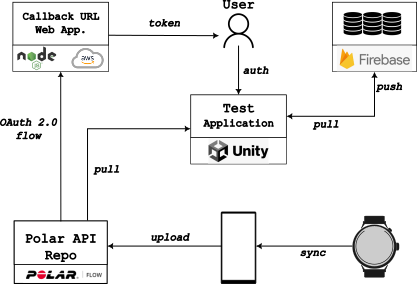
\includegraphics{images/architecture.png}
        \caption{System Architecture}
        \label{fig:architecture}
        \centering
        \end{figure}

    
    \section*{Schedule of work}
    \printbibliography


\end{document}
